\documentclass{article}

\usepackage{arxiv}

\usepackage[utf8]{inputenc} % allow utf-8 input
\usepackage[T1]{fontenc}    % use 8-bit T1 fonts
\usepackage[hidelinks]{hyperref}       % hyperlinks
\usepackage{url}            % simple URL typesetting
\usepackage{booktabs}       % professional-quality tables
\usepackage{amsmath,amssymb,amsthm}
\usepackage{amsfonts}       % blackboard math symbols
\usepackage{layouts}
\usepackage{microtype}      % microtypography
\usepackage{mathrsfs}
\usepackage{nicefrac}       % compact symbols for 1/2, etc.
\usepackage{graphicx}
\usepackage{doi}
\usepackage{listings}
\usepackage{tikz}
\usepackage[backend=biber,style=ieee]{biblatex}

\addbibresource{references.bib}

\usetikzlibrary{trees}

\title{Rust for Scientific Computing}

%\date{September 9, 1985}    % Here you can change the date presented in the paper title
%\date{}                     % Or removing it

\author{
    \href{https://orcid.org/0009-0001-0613-7978}{
        
\includegraphics[scale=0.06]{orcid.pdf}
        \hspace{1mm}Jonas Pleyer
    }
    \thanks{
        \href{https://jonas.pleyer.org}{jonas.pleyer.org}
    }\\
    Freiburg Center for Data-Analysis and Modeling\\
    University of Freiburg\\
    \texttt{jonas.pleyer@fdm.uni-freiburg.de}
    % \\
    %% examples of more authors
    % \And
    % \href{https://orcid.org/0000-0002-6371-4495}{
    %     
\includegraphics[scale=0.06]{orcid.pdf}
    %     \hspace{1mm}Christian Fleck
    % }\\
    % Freiburg Center for Data-Analysis and Modeling\\
    % University of Freiburg
}

% Uncomment to remove the date
%\date{}

% Uncomment to override  the `A preprint' in the header
\renewcommand{\headeright}{Preprint}
%\renewcommand{\undertitle}{Technical Report}
\renewcommand{\shorttitle}{Rust for Scientific Computing}

\usepackage{enumitem}
\setlist{nolistsep}

%%% Add PDF metadata to help others organize their library
%%% Once the PDF is generated, you can check the metadata with
%%% $ pdfinfo template.pdf
\hypersetup{
    pdftitle={Rust for Scientific Computing},
    pdfsubject={q-bio.NC, q-bio.QM},
    pdfauthor={Jonas Pleyer, Christian Fleck},
    pdfkeywords={},
}

% Change numbering of equations
% \numberwithin{equation}{section}

% MAKE TITLES IN THEOREMS BOLD
\makeatletter
\def\th@plain{%
    \thm@notefont{}% same as heading font
    \itshape % body font
}
\def\th@definition{%
    \thm@notefont{}% same as heading font
    \normalfont % body font
}
\makeatother

\begin{document}
\maketitle

%###################################################################################################
\begin{abstract}
\end{abstract}

\pagebreak
\tableofcontents

\twocolumn
\pagebreak

\printinunitsof{in}\prntlen{\columnwidth}

% keywords can be removed
\keywords{Rust \and HPC \and Scientific Computing \and Programming}

%###################################################################################################
\section{Introduction}

% General Remarks about languages
% \begin{enumerate}
%     \item Programming languages allow us to express machine instructions in human-readable code.
%     \item Depend on use-case
%     \item Translate human-interpretable code into machine instructions
%     \item tradeoff between high-level view (abstraction) and performance (low level)
%     \item C++ has "zero-cost" abstractions
% \end{enumerate}

Programming languages sit at the heart of all things computation.
They allow users to express higher-level instructions in a human-readable fashion such that this
code can be translated into machine-level instructions by either compiling or interpreting it.
Various classes of programming languages have emerged that serve distinct purposes.
Fundamentally, they aim to descibe problems at various levels of depth which allows humans to
interpret and reason about the executed instructions and therefore express their desired actions
more clearly.

Importance of programming in science
\begin{enumerate}
    \item New fields of study (computational physics, chemistry, biology, sociology, etc.)
    \item Cite some groundbreaking examples which were possible due to programming in
        science (maybe weather)
    \item
\end{enumerate}

Many languages have been devised to target specific realms which have emerged over the past decades.
They span across a range of abstraction levels, ranging from low-level languages to high-level ones.
The low-level operations level mostly deals with instructions on a level close to the actual
hardware such as memory allocation, pointer arithmetic or by using assembly instructions directly.
Meanwhile, high-level operations usually combine many lower-level ones to perform a single task.
An example for a high-level operation would be the addition of two matrices which might allocate the
required memory, fill it according to the given values and then call the appropriate math function
to pairwise add their entries.
Languages which can operate effectively on a lower level often bear the most promise for maximum
performance which is crucial in any scientific application.
These languages are mostly compiled using an optimizing compiler which enables many of their
performance achievements.

This mini-review concerns itself with the Rust programming language and aims to provide an overview
of the field of scientific computing with the Rust ecosystem.
Other systems programming languages  such as C, C++ or Fortran have dominated the field over the
past decades.
Most notably, C++ has been influential in establishing a model of "zero cost abstractions" where a
phrasing of the problem from a higher point of view does not involve any additional execution cost
but is handled by the compiler.
These and many other principles have allowed for a plethora of 

Judging C/C++
\begin{enumerate}
    \item Previous Decades: C/C++ in science
    \item Limitations of design choices of language become evident
    \item fragmented ecosystem; good for competition; bad for developer experience
    \item modern features missing: package manager with package registries, build system
    \item technical details; mutable by default, templates vs generics, backwards
        compatiblity becomes a
        problem ("there is a much simpler langauge within C++ that tries to get out"),
        macros, no clear
        ownership rules on a language level, dangling pointers
    \item still many good principles (such as RAII) and design principles/concepts (cite
        gang of four)
\end{enumerate}

The need for modern languages
\begin{enumerate}
    \item Java aimed to replace C due to pointers
    \item Go also aims to replace it, go is garbage-collected; thus cannot be as
        well-performing as C++ or C
    \item Python, Javascript for high-level abstractions ("as glue"); no performance howerver
\end{enumerate}

Elaborate on why Rust solves many problems
\begin{enumerate}
    \item safety guarantees; ensures that code which we write actually performs what we
        set out to do
    \item no dangling pointers
    \item zero-cost abstrations
    \item compiled without garbage-collector
    \item tooling: modern ecosystem; package manager, build system, package registry
    \item strong type system which is generally considered sound
    \item macro system gets type-checked
    \item very good C-interop; utilize existing software
\end{enumerate}

Show that many companies are starting to adopt Rust
\begin{enumerate}
    \item Amazon (AWS)\\ AWS developed Firecracker, a microVM monitoring service powering
        AWS Lambda and AWS
        Fargate. Firecracker is built primarily in Rust to offer fast cold boot times and
        secure workload
        isolation.
    \item Rust-supported runtimes like AWS Lambda also allow developers to write
        serverless functions using
        Rust.
    \item Google\\ Fuchsia, Google's modern operating system, uses Rust extensively for
        system components
        such as drivers and services to enhance security and reliability.
    \item Google (Android)\\ Android integration: Rust has been adopted within the
        Android Open Source
        Project (AOSP) to improve memory safety in critical system components. DEV
        Community Litslink
    \item Meta (Facebook)\\ Mononoke, Facebook’s large-scale source control backend for
        Mercurial, was
        written in Rust to improve performance and reliability in its monorepo.
    \item Meta (Facebook)\\ Facebook employs Rust in developing CLI tools, distributed
        systems, and cron
        jobs. Engineers write millions of lines of Rust internally.
    \item Apple\\ Apple’s Cloud Traffic team and backend infrastructure have been
        shifting from C to Rust,
        with new functionality being primarily built in Rust. This change was driven by performance,
        security, and developer efficiency goals. Reddit
    \item Microsoft\\ Although not part of FAANG, it’s noteworthy—Microsoft is rewriting
        parts of the Windows
        kernel and system components in Rust (e.g., DWriteCore, GDI Regions),
        prioritizing memory safety.
    \item Azure services-like Azure IoT Edge—also incorporate Rust.
    \item Linux Kernel\\ Only other supported language except from C
\end{enumerate}

\begin{figure*}
    \centering
    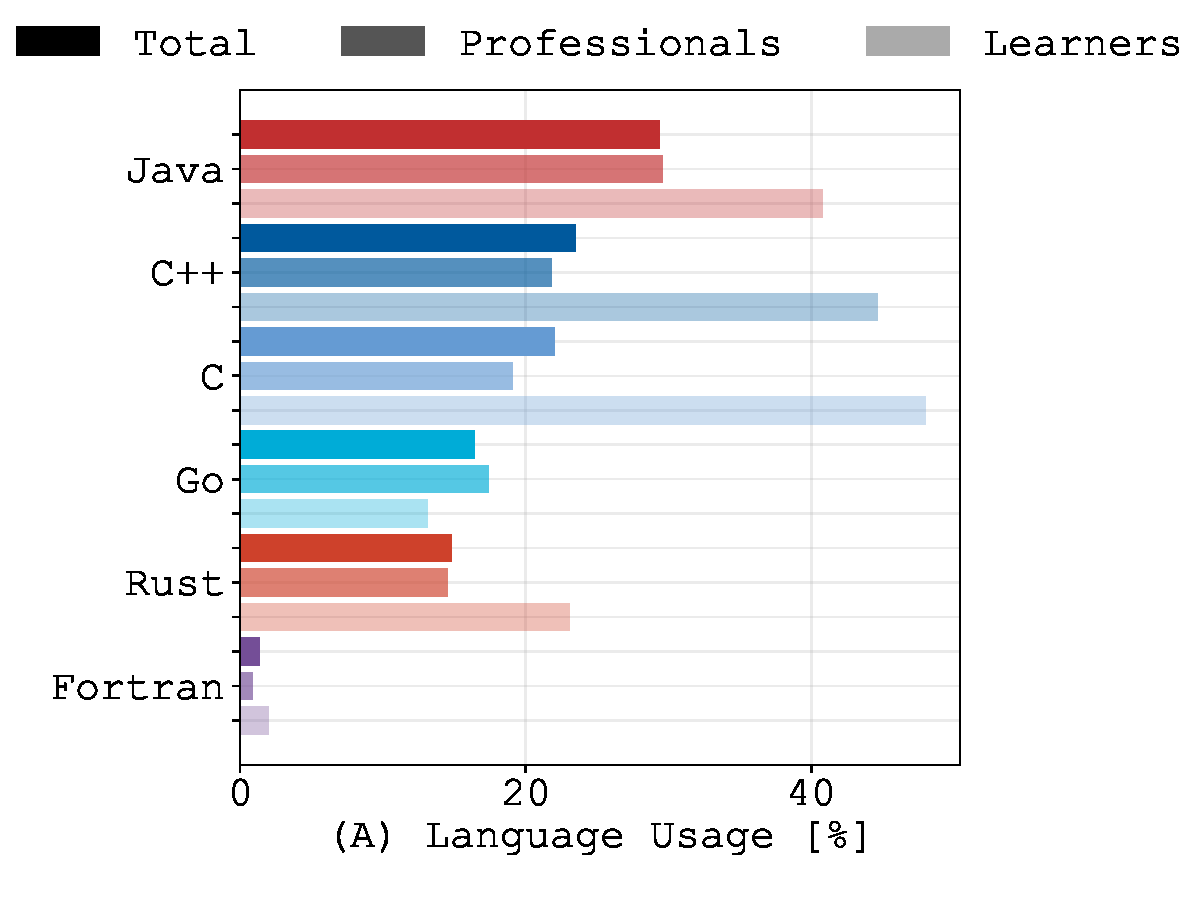
\includegraphics[width=0.5\textwidth]{figures/stackoverflow-popular-languages.pdf}%
    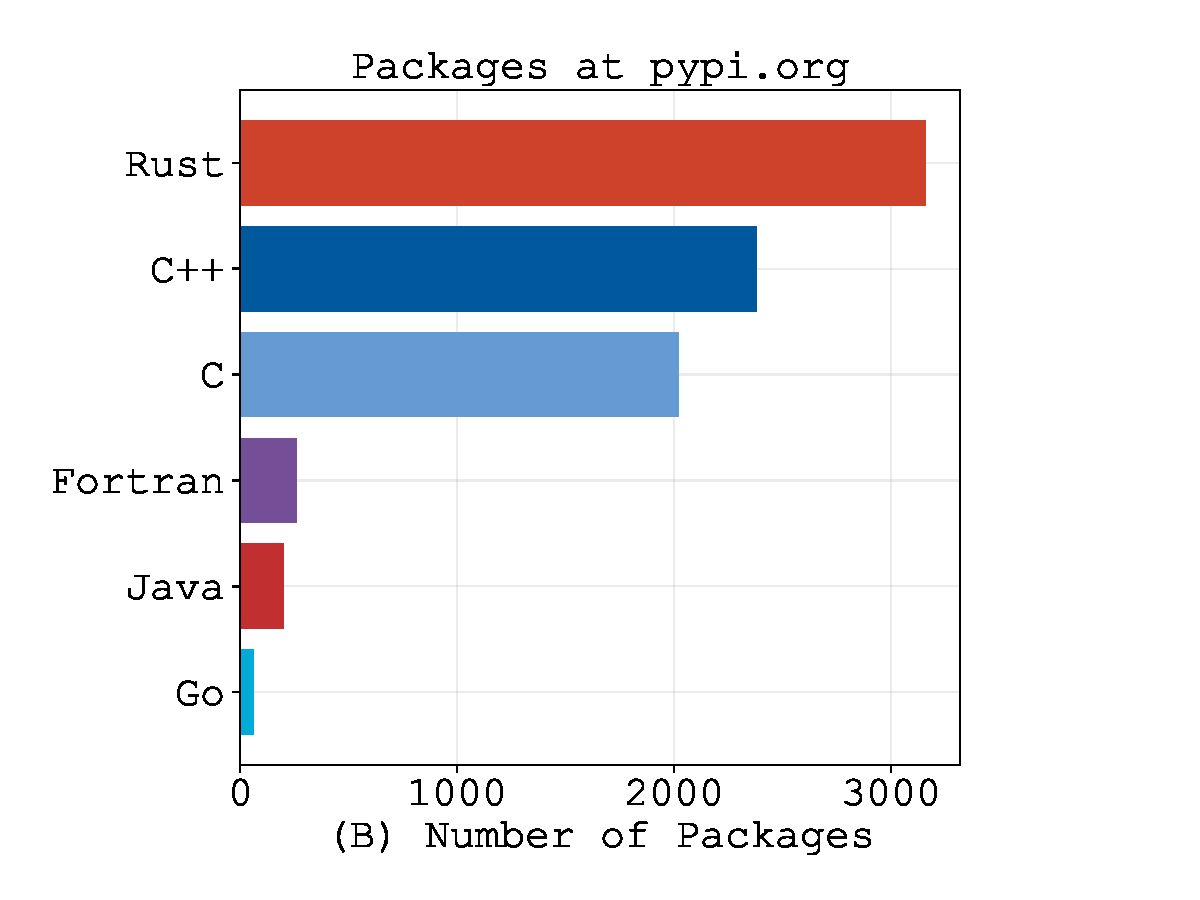
\includegraphics[width=0.5\textwidth]{figures/pypi-org-used-languages.pdf}
    \caption{
        Usage of programming languages according to (A) stackoverflow.com and (B) pypi.org.
    }
\end{figure*}
\begin{figure*}
    \centering
    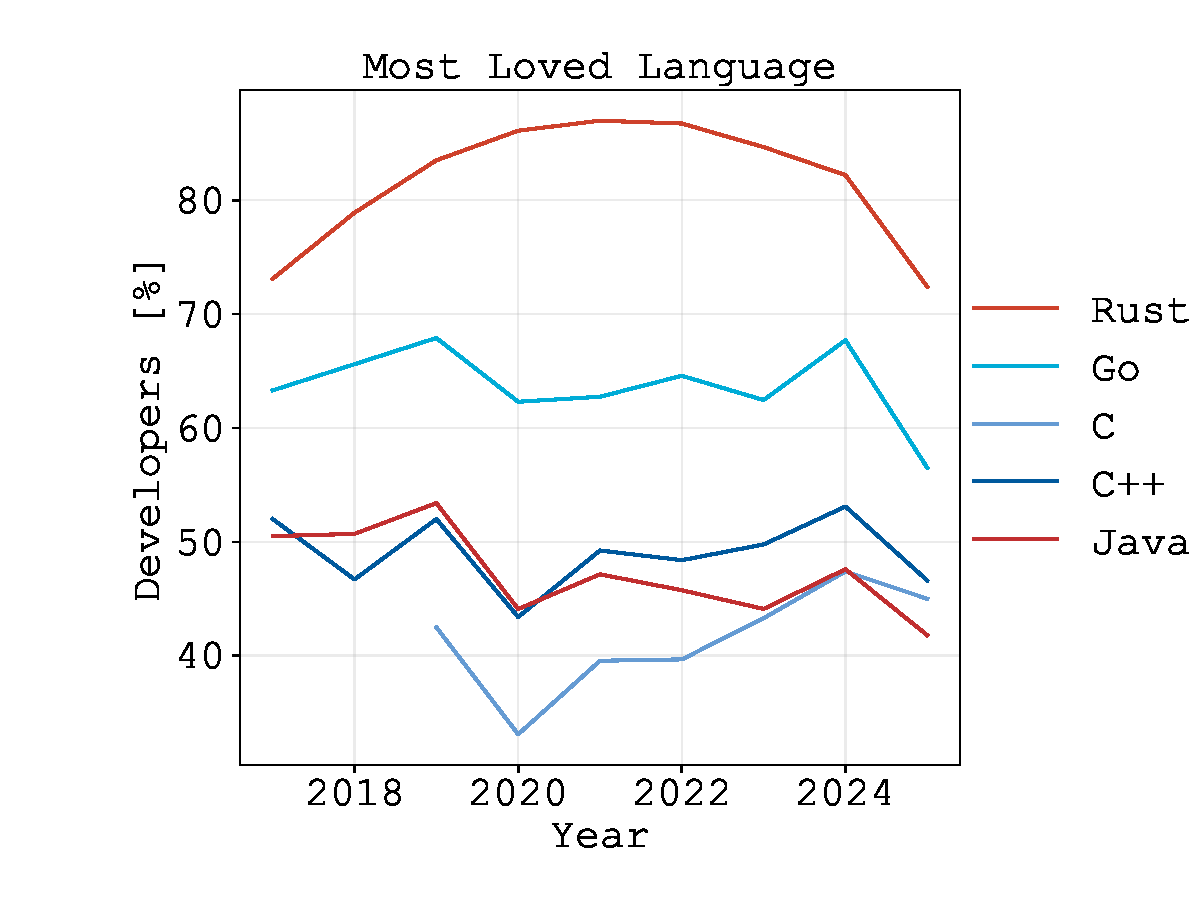
\includegraphics[width=0.5\textwidth]{figures/stackoverflow-loved-language.pdf}%
    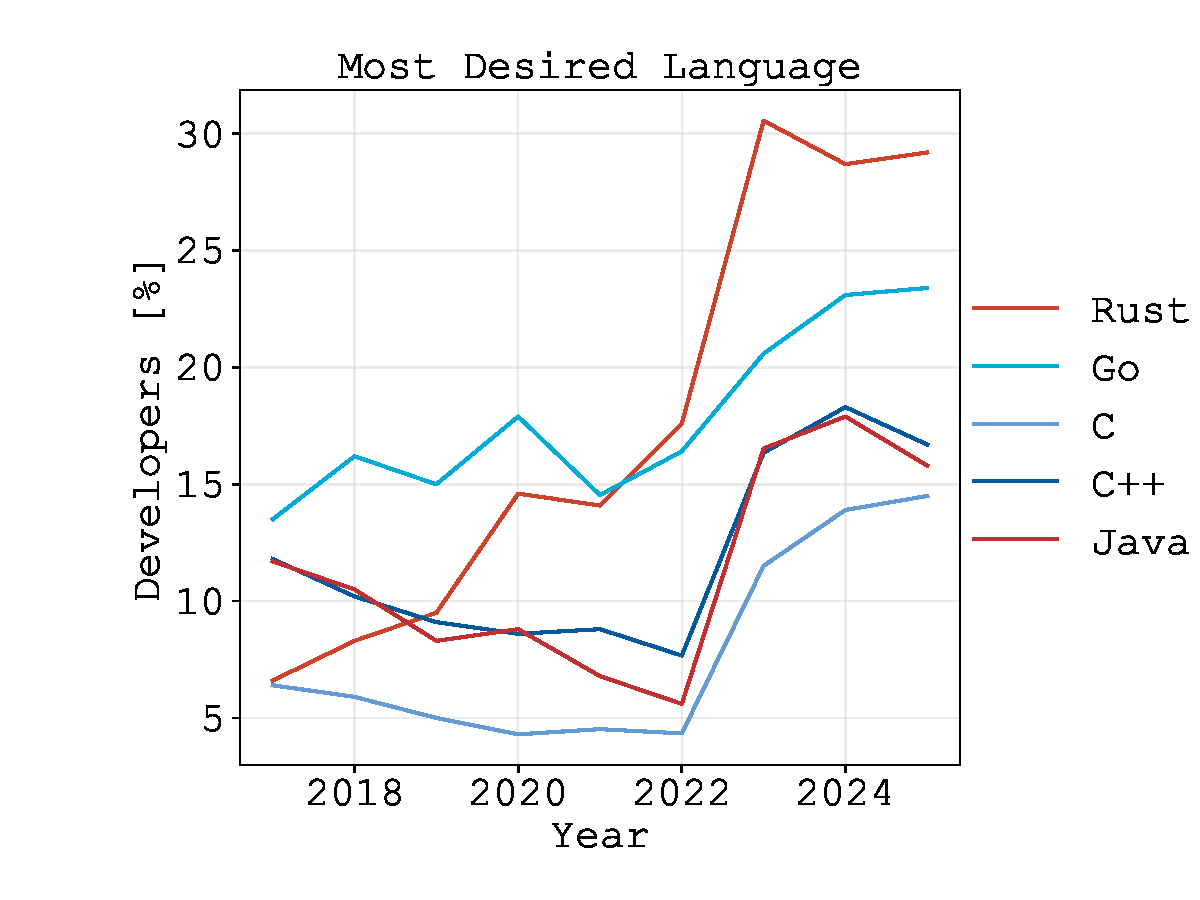
\includegraphics[width=0.5\textwidth]{figures/stackoverflow-desired-language.pdf}
    \caption{
        Popularity of the Rust programming language.
    }
\end{figure*}
\begin{figure*}
    \centering
    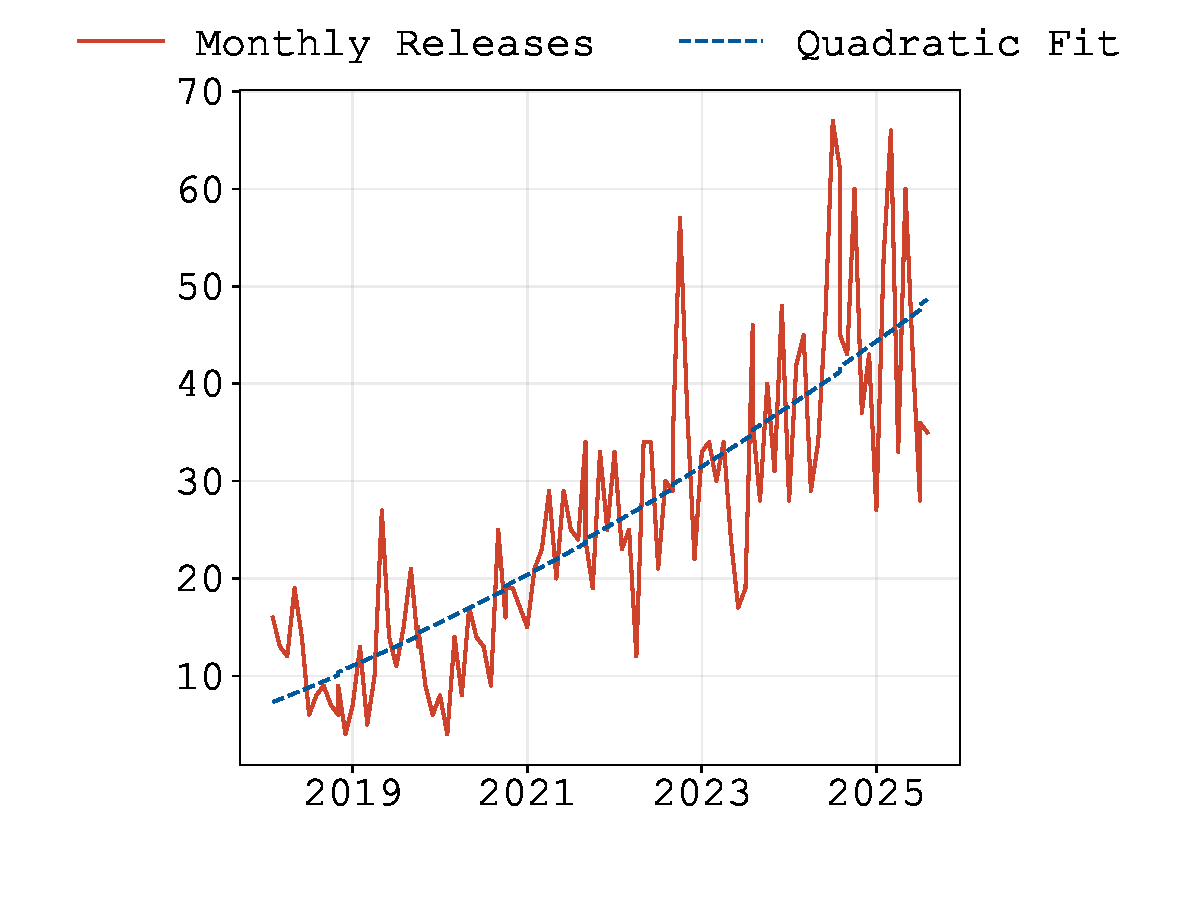
\includegraphics[width=0.5\textwidth]{figures/crates-io-release-numbers.pdf}%
    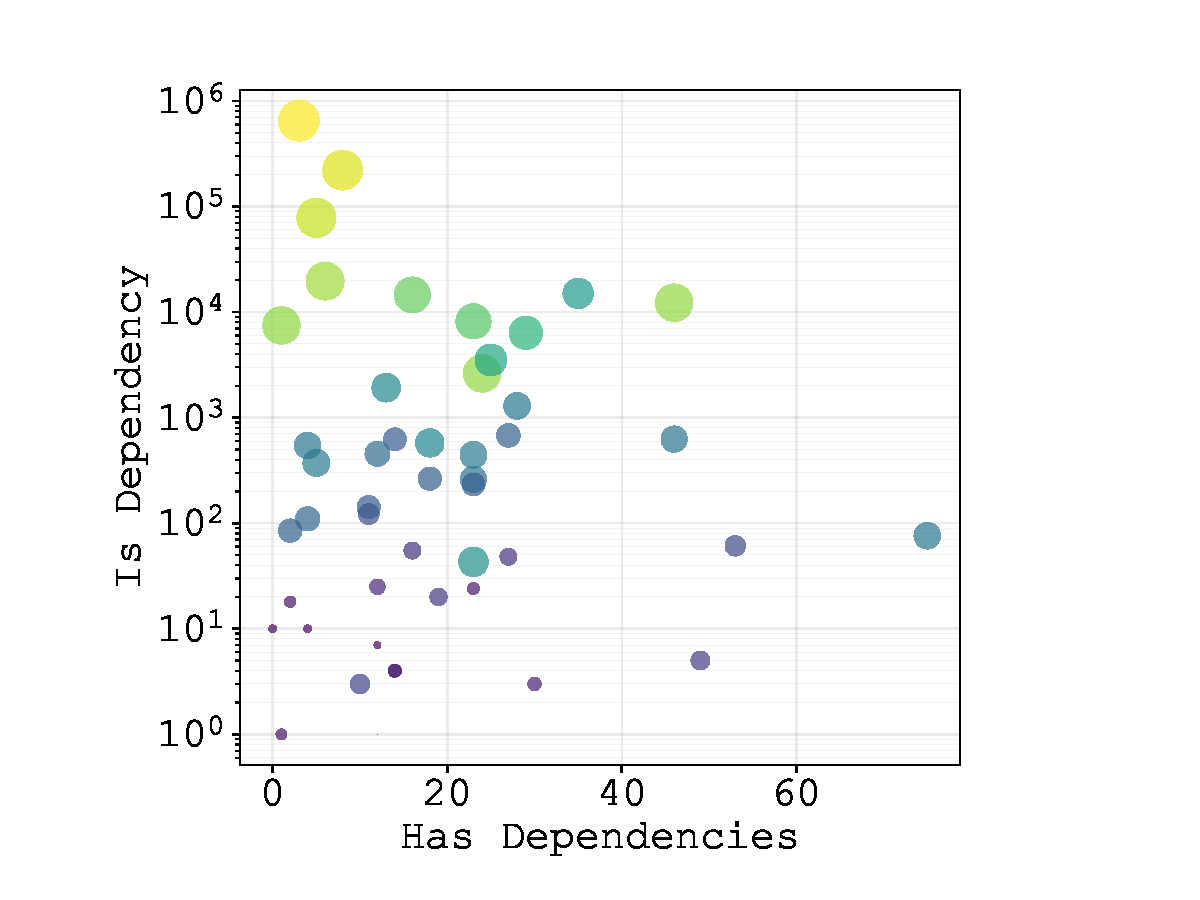
\includegraphics[width=0.5\textwidth]{figures/crates-io-deps-downloads-scatter.pdf}
    \caption{
        Number of releases of all included crates.
        Measure of overall growth of the field.
        The second figure can be misleading since this will for example not capture the setup where
        a crate is the dependency of a pypi.org package which is downloaded very often.
        The colors and size of the markers are also scaled logarithmically with the number of total
        downloads.
    }
\end{figure*}

%###################################################################################################
\section{Ecosystem and Libraries}

\begin{table*}
    \centering
    \begin{tabular}{l r r r r r}
        \toprule
        Crate Name &Last Update &Version &$N_d$ &$D_\text{week}$ &$D_\text{total}$\\
        \midrule
        Lamellar         &2025-03-31 &0.7.1      &42   &20       &     16.9k\\
        argmin           &2024-02-27 &0.10.0     &18   &12003    &   1227.7k\\
        arrow            &2025-08-25 &56.1.0     &23   &7532     &  27425.0k\\
        bevy             &2025-05-30 &0.16.1     &35   &10175    &   2847.7k\\
        bless            &2025-07-20 &0.1.1      &13   &80       &      0.6k\\
        burn             &2025-07-18 &0.18.0     &12   &1793     &    319.7k\\
        c3dio            &2024-04-08 &0.8.0      &2    &24       &     11.8k\\
        cargo-upgrades   &2025-08-25 &2.2.4      &10   &553      &     64.7k\\
        cellular\_raza   &2025-08-05 &0.3.0      &10   &157      &     27.4k\\
        cfsem            &2025-08-14 &2.5.0      &8    &106      &      4.9k\\
        city2ba          &2020-02-28 &1.1.0      &20   &19       &      3.0k\\
        cmake            &2025-02-10 &0.1.54     &1    &899615   &  91211.9k\\
        cudarc           &2025-08-07 &0.17.2     &5    &1184     &    647.0k\\
        cxxbridge        &2019-12-28 &0.0.0      &0    &14       &      1.3k\\
        deimos           &2025-06-23 &0.10.0     &13   &40       &      7.1k\\
        diffsol          &2025-07-16 &0.6.6      &16   &131      &     33.9k\\
        dioxus           &2025-08-11 &0.6.3      &28   &         &    637.5k\\
        egobox           &2025-08-22 &0.32.0     &18   &250      &     35.6k\\
        enzyme           &2021-12-26 &0.4.0      &5    &17       &      5.4k\\
        extendr-api      &2025-07-12 &0.8.1      &11   &968      &    178.4k\\
        factrs           &2025-01-13 &0.2.0      &20   &24       &      1.8k\\
        faer             &2025-04-29 &0.22.6     &46   &1322     &    528.4k\\
        faucet           &2025-05-31 &0.2.0      &7    &33       &      3.0k\\
        fem\_2D          &2023-04-20 &0.2.2      &6    &20       &      5.4k\\
        gcv\_spline      &2024-01-28 &0.2.0      &1    &16       &      2.5k\\
        \bottomrule
    \end{tabular}
    \caption{TODO}
\end{table*}

\subsection{Foundational Components}
Definition:\\
Lowest level of library considered in this review. Other crates depend on these
foundational crates.

\subsubsection{Linear Algebra \& Arrays}
(nalgebra, ndarray) (dense, sparse matrices, solvers)

\subsubsection{Numerical Methods}
(floating point arithmetic, etc.)

\subsubsection{Statistics \& Probability}
(statrs, ndarray-stats, smartcore)

\subsubsection{Symbolic \& Algebraic Computing}
(num, rug, speciyl, symcc, enzyme)

\subsubsection{Datastructures}
(graphs, etc.)

\subsection{Computational Methods}
Definition:\\
They are typically built on top of Foundational Components. Can also generalize over
many of these (such as different linear algebra crates).

\subsubsection{Optimization}
\subsubsection{Differential Equations}
(ODEs, PDEs)

ODE solvers~\cite{Renevey2024}, Diffsol

\subsubsection{Physics Engines}
(Fluid Dynamics, Manybody)

salva (2D \& 3D)~\cite{Crozet2024}

Rapier (2D \& 3D)~\cite{Crozet2025}

\subsubsection{Numerical Integration \& Differentiation}
(quadrature, monte-carlo, symbolic diff, enzyme)

\subsubsection{(Probabilistic Algorithms)}

\subsection{High-Performance \& Scalable Computing}
Definition:\\
Frameworks/libraries that allow greater scalability or usage of additional resources
such as GPUs/TPUs etc.

\subsubsection{Parallel Computing}
(rayon, compare to openmp, MPI bindings)

\subsubsection{GPU \& Accelerators}
(rust-cuda, cudarc, wgpu~\cite{Fitzgerald2025}, opencl, mention SPIRV)

\subsubsection{Sparse \& Structured Computations}
(large databases)

\subsection{Creature Comforts}
Definition:\\
Everything that is still missing

\subsubsection{Debugging}
(Rust Errors as values, tracing, logging) ecosystem

\subsubsection{Storage}
(serde, json, xml, ron, ...)

\subsubsection{Bindings}
(pyo3, maturin, C, cxxbridge, cmake)

\subsection{Visualization}
Definition:\\
Libraries which can be used to visualize results. (self-explanatory)

\subsubsection{Plotting (2D)}
plotters, plotlib, gnuplot bindings

\subsubsection{3D Rendering}
vtk-rs

Meshing (honeycomb) (maybe this should be in section "Computational Methods" / "Differential
Equations")

\subsubsection{Interactive}
(dioxus)

%###################################################################################################
\section{Applications}
\label{section:applications}

\subsection{Physics \& Engineering}
\subsection{Biology \& Chemistry}
\cite{Pleyer2024}, Computational Oncology~\cite{Köster2025}, Proteomics~\cite{Anechitoaie2024}
\subsection{Climate \& Earth Sciences}
\subsection{Economics \& Finance}
\subsection{Social Sciences}

%###################################################################################################
\section{Discussion}
\label{section:discussion}

\begin{itemize}
    \item Job Opportunities remain a problem in Rust
\end{itemize}

%###################################################################################################
\section{Conclusion}
\label{section:conclusion}

\onecolumn
\printbibliography

%###################################################################################################
\pagebreak
\newcounter{supplementSection}
\renewcommand{\thesubsection}{S\arabic{supplementSection}}
\newcommand{\supplement}[1]{%
    \stepcounter{supplementSection}%
    \subsection{#1}
}
\renewcommand{\thesection}{}

\section{Supplementary Material}
\supplement{List of all crates}

\paragraph{Scientific Computing in Rust monthly Newsletter}

approx-derive\\
A procedural macro that automatically implements approximate equality traits for
floating-point types and custom structs. It builds on the approx crate to make testing numerical
code easier. This helps ensure tolerance-based equality checks are consistent and less error-prone.

approxim\\
A library for approximation algorithms in numerical computing. It provides tools for
approximating functions, datasets, or computations efficiently. The focus is on balancing precision
with performance in scientific workflows.

bacon-sci\\
A scientific computing library built on Rust that provides a foundation for numerical
and algebraic operations. It aims to be a lightweight alternative to larger ecosystems. Its design
emphasizes safety, performance, and modularity.

cargo-upgrades\\
A Cargo subcommand for upgrading dependencies in a Rust project. It automates
version checking and updates Cargo.toml accordingly. This reduces the manual overhead of keeping
scientific projects up to date.

faer\\
A linear algebra library for Rust with focus on high-performance matrix operations. It
provides dense and sparse routines with attention to numerical stability. The crate aims to become
a foundation for scientific and machine-learning applications in Rust.

fact.rs\\
A crate for fast matrix factorizations and related linear algebra decompositions. It
provides algorithms like LU, QR, and eigenvalue methods. Its goal is to complement crates like faer
with specialized routines.

globalsearch\\
A Rust crate for global optimization and search algorithms. It supports solving
complex optimization problems where local minima are common. Useful in scientific simulations and
computational experiments.

indexing\_fmt\\
A utility crate for formatting indices and ranges in scientific computing contexts.
It makes working with slices and multi-dimensional arrays more ergonomic. This helps in debugging
and presenting results.

integraal\\
A symbolic and numerical integration library for Rust. It supports computing definite
and indefinite integrals for a variety of functions. Its goal is to provide a reliable integration
toolkit for researchers.

ndgrid\\
A crate for generating multi-dimensional grids, similar to MATLAB’s ndgrid. It is
especially useful in scientific computing for parameter sweeps and simulations. Provides ergonomic
grid construction for Rust’s array ecosystem.

ndelement\\
A crate for manipulating individual elements in multi-dimensional arrays. It offers
convenient indexing and iteration across dimensions. Designed to complement libraries like ndarray.

ndarray\\
A core Rust crate for n-dimensional arrays, inspired by NumPy. It provides efficient
array structures, broadcasting, slicing, and linear algebra support. Widely used as a foundation
for many Rust scientific computing libraries.

ploc\\
A parallelized algorithm library for localization and clustering tasks. Focuses on scalable
implementations of clustering approaches. Intended for large datasets in scientific applications.
\url{https://dotblocks.com/}

Quant-Iron\\
A crate for quantitative finance and scientific modeling. It implements financial
instruments, stochastic processes, and numerical solvers. Designed to bridge scientific computing
with financial applications.

paradis\\
A discrete dislocation dynamics simulator written in Rust. It is used in materials
science to model dislocation behavior under stress. The library emphasizes performance and
scalability for large simulations.

repgenerate\\
A tool for generating reproducible reports from computational experiments. It
integrates with Rust code to ensure scientific workflows can be repeated. Useful for open and
transparent research.

rsmpi\\
Rust bindings to the Message Passing Interface (MPI). It enables parallel computing across
distributed systems, a key component in HPC. Provides safe abstractions while maintaining low-level
control.

serde\\
A widely used Rust serialization and deserialization framework. It supports many formats
like JSON, YAML, and custom binary encodings. In scientific computing, it helps with data exchange
and configuration management.

sequenceprofiler\\
A bioinformatics library for profiling biological sequences. Provides tools for
analyzing DNA, RNA, or protein sequences. Aimed at high-performance sequence analysis in Rust.

zarrs\\
A Rust implementation of the Zarr data format for chunked, compressed N-dimensional arrays.
It allows efficient storage and manipulation of large scientific datasets. Especially useful in
machine learning and climate science.

\paragraph{JOSS}

fastatomstruct\\
A Rust library for high-performance analysis of atomic systems. It provides tools
for structural and dynamical computations, enabling simulations and data analysis in computational
chemistry and materials science. Optimized for speed, it can handle large datasets efficiently.

grepq\\
A Rust tool designed to process and filter FASTQ files efficiently. It matches sequences
against sets of regular expressions, making it useful for high-throughput sequencing data analysis.
Its focus is on speed and flexibility for genomic workflows.

pengWann\\
A library that computes chemical bonding descriptors using Wannier functions. It aids in
understanding electronic structure and bonding characteristics in materials. Suitable for quantum
chemistry and materials science applications.

wrenfold\\
A Rust library for symbolic computation and code generation tailored to robotics
applications. It allows automatic generation of control and kinematics code from symbolic
expressions. Supports efficient development of robotic algorithms.

kifmm-rs\\
A Rust framework implementing the kernel-independent fast multipole method (FMM). Used
to accelerate N-body computations in physics and engineering. Optimized for performance and
scalable to large simulations.

startinpy\\
A Python package for modeling and processing 2.5D terrains. Supports triangulated
meshes and geospatial analysis. Useful in geoscience, terrain analysis, and visualization.

Back to sequences\\
A tool for tracing the origins of k-mers in sequencing data. Helps analyze and
understand sequence composition and frequency. Useful for genomics and bioinformatics research.

sourmash v4\\
A bioinformatics toolkit for genome and metagenome analysis. Provides fast
comparison, search, and analysis of sequencing data. Supports scalable workflows with large
datasets.

extendr\\
A Rust library that facilitates seamless integration with the R programming language.
Allows calling Rust functions from R and vice versa. Focuses on performance and ease of use for
scientific computing.

Pywaterflood\\
A Python library for analyzing well connectivity in hydrogeology or petroleum
engineering. Uses capacitance-resistance modeling to simulate flow and connectivity. Supports
data-driven analysis for reservoir studies.

Gibbs Sea Water Oceanographic Toolbox\\
A Rust implementation of the TEOS-10 toolbox for
oceanographic computations. Provides tools for thermodynamic and salinity calculations in seawater.
Useful for oceanographers and climate researchers.

Raphtory\\
A toolkit for building and analyzing temporal graphs. Supports both Rust and Python
interfaces. Enables high-performance analytics on time-evolving network data.

HDT\\
A Rust library for working with HDT, a binary compression format for RDF data. Optimizes
storage and query of large knowledge graphs. Useful for semantic web and linked data applications.

egobox\\
A Rust toolbox for performing global optimization. Implements algorithms for efficiently
exploring high-dimensional spaces. Useful in engineering, machine learning, and simulation-based
optimization.

Fast k-medoids Clustering\\
A high-performance implementation of k-medoids clustering in Rust, with
Python bindings. Supports scalable clustering of large datasets. Ideal for machine learning and
data analysis tasks.

FEM\_2D\\
A Rust library for 2D finite element simulations. Supports hp-refinement for adaptive
mesh accuracy. Designed for engineering, physics, and numerical analysis applications.

retworkx\\
A Python graph library with Rust backend for performance. Supports graph creation,
traversal, and analysis. Useful in network science, bioinformatics, and algorithm development.

Rasusa\\
A bioinformatics tool for subsampling sequencing reads. Allows control of coverage in
genomic datasets. Helps optimize computational pipelines and reduce data size for analysis.

Sepia\\
A Rust tool for classifying sequencing reads by taxonomy. Provides high-performance
analysis for metagenomics studies. Helps researchers quickly categorize large datasets.

RustBCA\\
A Rust library implementing the binary collision approximation (BCA) for ion-material
simulations. Enables efficient modeling of particle interactions in materials. Used in physics and
materials research.

City2BA\\
A Rust package for generating synthetic bundle adjustment datasets. Useful in computer
vision and photogrammetry. Helps test and benchmark 3D reconstruction algorithms.

\paragraph{Scientific Computing in Rust 2025 talks}

stochastic-rs\\
stochastic-rs is a high-performance Rust library for simulating and analyzing
stochastic processes. Designed for applications in quantitative finance, AI training, and
statistical modeling, it provides efficient tools to generate synthetic data and analyze complex
stochastic systems.

Pixi\\
The missing companion to Cargo.

NPB-Rust\\
NAS parallel benchmarks in Rust. \cite{martins2025npbrustnasparallelbenchmarks}

cellular\_raza\\
Cellular agent-based modeling from a clean slate.

ORMATEX\\
Oak Ridge MATrix EXponential tools - methods to compute the matrix exponential

orbweaver-rs\\
A fast R library for working with Nodes in a graph.

triple-r\\
Recycle, Reuse, Reduce. triple-r is a high-performance Rust library that provides
wrappers around standard library collections to enable the reuse of their memory allocations. By
recycling the underlying memory of collections like HashMap and Vec, triple-r helps reduce
allocation overhead in performance-critical applications.

faucet (maybe remove; does this fit the scope?)\\
Scale, deploy and route Plumber APIs and Shiny
applications with ease and efficiency.

qoqo (Roqoqo)\\
A toolkit to represent quantum circuits by HQS Quantum Simulations.

ninterp\\
Numerical interpolation in N-dimensions.

Arrow\\
Arrow, Rust, and cross-language data science tooling.

eVaiutilities\\
A data management software for the analysis of the eVai output files. It allows the
analysis of the genomic variants further such as analyzing the multiple genomic annotated variants,
reference and alternate allele, enabling coordinate search, coordinate search with specified
variants and annotation search across a large number of population.

Honeycomb\\
Combinatorial maps implementation for meshing applications.

qhull-rs\\
Safe Rust Qhull bindings. Qhull computes the convex hull, Delaunay triangulation,
Voronoi diagram, halfspace intersection about a point, furthest-site Delaunay triangulation, and
furthest-site Voronoi diagram.

HULK (maybe out of scope?)\\
The robot control program and associated tools of the RoboCup SPL team
HULKs. \url{https://hulks.de/hulk/} "Rust’s safety and performance features benefit real-time
robotics, and the challenges of integrating it into an ecosystem traditionally dominated by C++ and
Python."

burn\\
Burn is a next generation Deep Learning Framework that doesn't compromise on flexibility,
efficiency and portability. \url{https://github.com/tracel-ai/burn}\\
Commercial

Diffsol\\
A crate for solving differential equations.

Deimos\\
Open-source scientific data acquisition \& laboratory controls.

\paragraph{Scientific Computing in Rust 2024 talks}

oxidicom\\
A high-performance DICOM receiver for the ChRIS backend (CUBE).
\url{https://chrisproject.org/} ChRIS is an open-source platform for computational research and
medicine.

AcoDyn\\
Fluid dynamics on the GPU powered by Rust.

rlst\\
The Rust Linear Solver toolbox is an in-development project for dense and sparse linear
algebra routines in Rust.

Bless\\
Transparently logging program outputs.

cfsem\\
Quasi-steady electromagnetics including filamentized approximations, Biot-Savart, and
Grad-Shafranov.\\
\url{https://cfs.energy/} Commercial

sophus-rs\\
A fast electromagnetics library with Rust and Python.

Argmin\\
Rootfinders for Rust.

Rstats\\
Multidimensional data analysis in Rust.

Symbolica\\
Symbolica is a blazing fast computer algebra system for Python and Rust, born of a need
to push the boundaries of computations in science and enterprise.

rsrs (no crate, just github repo)\\
An implementation of the randomised strong recursive
skeletonisation

bevy\\
Bevy is a refreshingly simple data-driven game engine built in Rust.

Polars\\
Polars is a DataFrame library for Rust. It is based on Apache Arrow’s memory model. Apache
Arrow provides very cache efficient columnar data structures and is becoming the defacto standard
for columnar data.\\
A fast DataFrame library for Rust, with APIs also available in Python. It
provides powerful data manipulation, joins, and group-by operations with performance close to
Apache Arrow. Designed for data science, analytics, and scientific workflows.

Perpetaul\\
Perpetaul: a hyperparameter-free gradient boosting machine.

Biomechanics Foundation\\
Back to basics: rebuilding computational biomechanics crate by crate.
Many crates (maybe just cite one crate):
\begin{itemize}
    \item chiron - Graphical and command-line interface tools for Biomechanics Foundation
    \item gcv\_spline - Generalized Cross-Validated Splines for Interpolation and
        Derivation in Pure Rust
    \item onager - Featherstone rigid-body physics library built in Rust
    \item c3dio - A c3d parser, writer and editor written in Rust.
    \item bevy\_c3d - A .c3d asset loader plugin for the Bevy engine.
    \item Mannequin - Methods for kinematics and rigging, and dynamics in biomechanics
        applications and
        animation
    \item hominem - Biomechanical muscle models for simulating human motion
\end{itemize}
\url{https://biomechanicsfoundation.org/}
\url{https://github.com/biomechanics-foundation}

\#[offload] (feature draft)\\
New rustc feature called \#[offload], which allows running almost arbitrary Rust code on
co-processors like a GPU, TPU, or IPU
\url{https://github.com/rust-lang/rust/pull/145768}

Bempp-rs\\
Writing a grid library for finite and boundary element methods. \cite{Witherden2015}

\paragraph{Scientific Computing in Rust 2023 talks}

jiro\_nn\\
Low-friction high-detail Deep Learning framework in Rust

struqture\\
Represent quantum mechanical operators, Hamiltonians and open quantum systems.
\url{https://quantumsimulations.de/}

salso, caviarpd, \& fangs\\
R extensions written in Rust

Lamellar\\
A Rust-based asynchronous tasking and PGAS runtime for high-performance computing.

Sage\\
Enables fast proteomics searching and quantification at scale.

Bernstein–Bézier\\
Finite elements for RMM in Rust~\cite{Sky2024}

mwa\_hyperdrive\\
Calibration software for the Murchison Widefield Array (MWA) radio telescope.
\url{https://mwatelescope.github.io/mwa_hyperdrive/index.html}

alg\_tools\\
utility routines and tools for implementing iterative algorithms and (abstract)
numerical computing in Rust~\cite{Valkonen2023}. \url{https://tuomov.iki.fi/software/alg_tools/}

clarabel\\
Clarabel is an interior point numerical solver for convex optimization problems using a
novel homogeneous embedding~\cite{Clarabel_2024}.

fips\\
\cite{jeggle2023genericframeworkdataracefreemanyparticle}
\url{https://zenodo.org/records/6757615}

Lace\\
Bayesian tabular data analysis for Rust (and Python).

Rudolph\\
Improving productivity of medical research with Rust CLI tools.

Rusph\\
Rusph: a SPH astrophysical simulation code in the Rust programming language.

Roxido\\
Developing Rust-based R packages using the Roxido framework.

\end{document}
